\vspace*{1.5pc}

As the general relativity description of the spacetime metric historically engrained into the roots of modern observational cosmology, there was a divide as to the driving force responsible for the expansion. One school of thought put forth the \emph{steady state} model, in which the density of matter remains unchanged in the expanding Universe due to a steady homogenous creation of matter. The other school of thought, which would ultimatly prevail, proposed the \emph{Hot Big Bang} model, in which the matter density monotonically decreases as the scale factor increases. Consequently, the Universe was denser and hotter at earlier times, which I detailed in Sec.~\ref{sec:thermal}. In this section, I break down the main components of the cosmological fluid that obey Friedmann's equations. 


\subsection{Non Particular Components}

First shall be specified two components of the cosmological fluid that are not made of particles, but oddly have a defined energy density: the global curvature of the Universe and the cosmological constant. 

\subsubsection{Curvature}

From cosmological observation, it appears that the Universe has a global flat spatial geometry. Setting $\kappa=0$ in the first Friedmann equation defines the cosmological fluid's critical density $\rho_{\mathrm{cri}}$: \\
\begin{empheq}[box=\mymath]{equation}
\rho_{\mathrm{cri}}(t) = \frac{3H^2(t)}{8 \pi G}
\end{empheq} \\ with today's value being $\rho_{\mathrm{cri},0} = 8.293 10^{-11} h^2 ~\mathrm{eV}^4$ (see Appendix~\ref{apx:units} for expressing physical quantities in units of $h_p$, $k_b$ and $c$). In units of this critical density, the Friedmann equation can be written in compact form \\
\begin{equation}
\label{def:omega}
\rho(t) = \Omega(t) \times \rho_{\mathrm{cri}} (t)
\end{equation} \\ where the cosmological fluid is an admixture of radiation, non-relativistic matter and a curvature density \\
\begin{equation}
\rho_\kappa(t) = - \frac{3 \kappa}{8 \pi G} \frac{1}{a^2(t)}
\end{equation} \\ so that \\
\begin{equation}
\label{eq:rho_tot_def}
\rho(t) = \sum_{\alpha \in \lbrace r,m,\kappa \rbrace} \rho_\alpha (t) = \sum_{\alpha \in \lbrace r,m,\kappa \rbrace} \Omega_\alpha (t) ~ \rho_{\mathrm{cri}} (t)
\end{equation} \\ The curvature density is not a physical quantity. However, from Eq.~\ref{eq:rho_tot_def}, one can interpret it as the energy density that exceeds or is deficient with regards to the critical value that would make the Universe flat. In all that follows, I work under the assumption that $\kappa = 0$, and drop any contribution of $\rho_\kappa$ into Friedmann's equations.

\subsubsection{Dark Energy or Cosmological Constant}

Hubble diagrams of distant objects provided in the late 90's evidence for a negative value of the deceleration parameter $- \ddot{a}a/\dot{a}^2$, which appears under another normalisation as the second order term in Eq.~\ref{def:deva}. In other words, the expansion of the Universe was not decelerating as would be the case if the expansion was driven solely by the matter and radiation density; it was in fact doing just the opposite. \\

Because both the Einstein and metric tensors are divergencefree, one can incorporate a so-called \textbf{cosmological constant} $\Lambda$ into the Einstein tensor ($\pmb{G} \mapsto \pmb{G} - \Lambda \pmb{g}$) and verify the Einstein field equations: \\
\begin{equation}
\label{eq:EFE_contracted}
G_{\mu \nu} - \Lambda g_{\mu \nu} = 8 \pi G T_{\mu \nu}
\end{equation} \\ In this context, the $\Lambda$ scalar is uniform in space (although not necessarily in time) and acts as a ``drain'' term in spacetime warping. Another possible interpretation for the accelerated expansion of the Universe comes from incorportating it into the energy-stress tensor instead: $\pmb{T} \mapsto \pmb{T} + \Lambda \pmb{g}$, making it a ``source'' term in energy density, called \emph{dark energy}. In that case, this additional term can be thought of as a fluid whose equation of state is \\
\begin{empheq}[box=\mymath]{equation}
w_\Lambda = -1
\end{empheq} \\ In other words, the more you compress it, the less dense it gets. Inversely, as the Universe expands and the cosmological fluid dilates, the dark energy component exerts growing pressure on its surroundings and drives the expansion ever so further. It goes without saying that there are currently no known material on Earth displaying such a counter-intuitive property. It is still to this day unclear which of these two interpretations --- as a dark energy in $\pmb{T}$ or a cosmological constant in the EFEs --- is correct, if any one of them at all, since both of them involve a standing mystery as to its nature, behavior and origin. \\

\begin{figure}[!]
\begin{center}
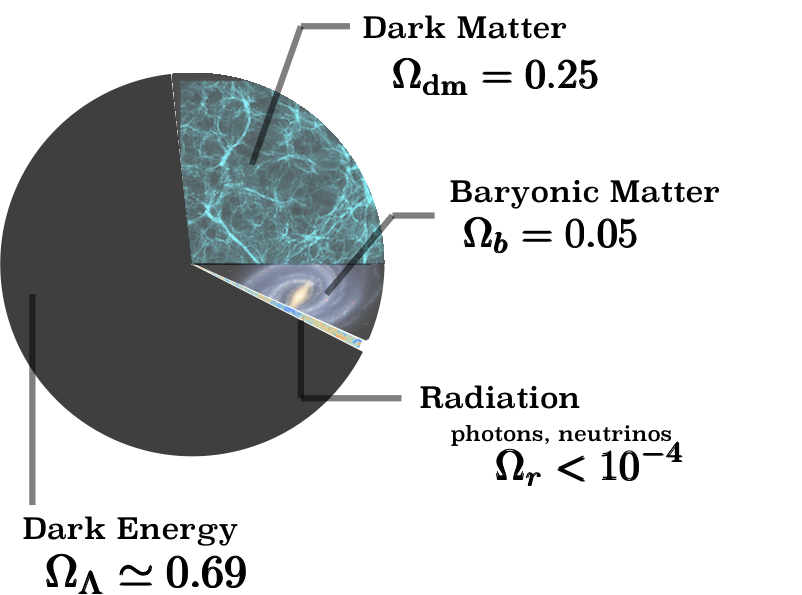
\includegraphics[width=0.65\columnwidth]{darkside.png}
\caption{Relative abundance in terms of energy density of the main components of the Universe today ($z=0$).}
\end{center}
\label{fig:camembert}
\end{figure}


The total energy density in units of critical density must therefore be written

\begin{equation}
\Omega_r + \Omega_m + \Omega_{\Lambda} = 1 - \Omega_{\kappa}
\end{equation} with $\Omega_\kappa = 0$ for a flat Universe. This expression introduces the quantity
\begin{equation}
\label{eq:rhode}
\rho_\Lambda = \frac{\Lambda}{8 \pi G}
\end{equation} which is derived from the Friedmann equations with Eq.~\ref{eq:EFE_contracted} as the expression of the EFEs. This quantity being homogenous to an energy density, it follows that in the cosmological constant interpretation of the acceleration of the Universe's expansion, $\Lambda$ has dimentions of the inverse of a surface. Several cosmological probes either measure independantly or infer $\Omega_\Lambda \sim 0.7$ today. Throughout this work, I used the value \\
\begin{empheq}[box=\mymath]{equation}
\label{eq:omega_lambda}
\Omega_\Lambda = 0.69
\end{empheq} \\ consistent with the best fitted value from the Planck collaboration's analysis on the cosmic microwave background temperature anisotropies. Notice from Eq.~\ref{eq:rhode} that the energy density associated with $\Lambda$ (or dark energy, which I'll use interchangeably throughout this thesis) is only implicitely dependant on time through $\Lambda$'s own time dependance. In the benchmark cosmological model, $\Lambda$ is deemed a constant in both space and time, and so $\rho_\Lambda \propto a^0$. In a $\Lambda$ dominated Universe, which applies to the current state of the Universe, the first Friedmann equation simplifies to \\

\begin{equation}
\label{eq:Friedmann_LDE}
\left( \frac{\dot{a}}{a} \right)^2 \simeq \Omega_\Lambda
\end{equation} \\ which integrates into $a(t) \propto \exp\left[ H_0 \Omega_\Lambda^{1/2} t \right]$, or, using conformal time, $a(\tau) \propto (-\tau)^{-1}$.

\subsection{Inventory of Radiation}
\label{sec:radiation}

With the non-particular components of the cosmological fluid out of the way, we can instantiate the relativistic matter population, which in sum total has an energy density of

\begin{empheq}[box=\mymath]{equation}
\label{eq:omega_radiation}
\Omega_{r,0} = 8.24 \times 10^{-5}
\end{empheq} \\ critical densities. The only relativistic species today are (1) photons from the cosmic microwave background, (2) massless\footnote{by massless I mean any neutrino mass eigenstate lighter than $10^{-4}~\mathrm{eV}$} neutrinos from the cosmic neutrino background, and (3) any hypothetical light thermal relic; all three of which I detail in the subsections below.


\subsubsection{The Cosmic Microwave Background}

\begin{figure}
\begin{center}
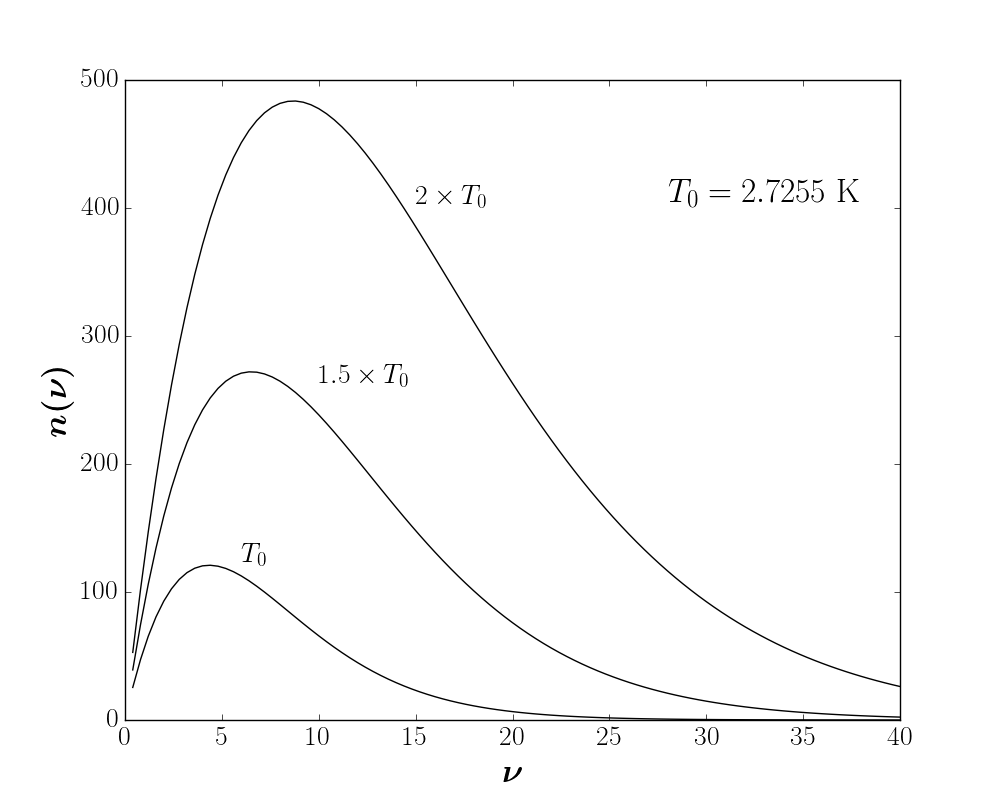
\includegraphics[width=0.75\columnwidth]{photon_eq.png}
\caption{energy density per unit of frequency of photons in thermal equilibrium as a function of frequency given by Eq.~\ref{eq:Fermi_photon} for 3 temperatures. Units are arbitrary.}
\label{fig:planck_eq}
\end{center}
\end{figure}

Up until recombination, the rate of expansion was significantly weaker than the scattering interaction rate between photons and free electrons $H(t) \ll \Gamma_{\mathrm{Compton}}$. This thermal equilibrium defines its black body temperature $T_\gamma$. Since photons have no chemical potential, 
\begin{equation}
\label{eq:Fermi_photon}
n_{\gamma} (E) dE \propto \frac{E^2 dE}{e^{E / k_b T_\gamma} - 1}
\end{equation} with $dE = h d\nu$ the energy interval and $\nu$ the photon frequency. The energy density of photons is therefore proportional to the 4th power of its black body temperature, known as \emph{Stefan's Law} \\
\begin{equation}
\label{eq:photon_rho}
\rho_\gamma c^2 = \int_0^\infty E dE~n(E) = \frac{8 \pi^5}{15} \frac{k_b^4}{15 h^3 c^3} ~ T_\gamma^4
\end{equation} \\ which is conformal to the expression in Eq.~\ref{eq:relmat} for bosons with $g=2$ (there are two spin states). The energy of a photon is inversely proportional to its wavelength $\lambda = \hbar c / k_b T_\gamma \propto a(t)$ which scales as the scale factor. This implies that the evolution of temperature with the scale factor is 
\begin{equation}
\label{eq:T_f_a}
T(t) = \frac{T_0}{a(t)}
\end{equation} As the Universe expands, the energy density of photons is therefore diluted by this $a^{-1}$ factor pertaining to its energy in addition to the $a^{-3}$ factor pertaining to the dilution of volume, as illustrated in Fig.~\ref{fig:expa}. At any point in time $t$, the energy density is therefore \\

\begin{equation}
\label{eq:rho_photon_f_a}
\rho_\gamma (t) = \rho_\gamma^0 ~\left( \frac{a_0}{a(t)} \right)^4
\end{equation} \\ with $\rho_{\gamma, 0}$ its current value. \\

As the background temperature falls below the binding energy of the Hydrogen atom, electrons progressively bound to protons. Once recombination is complete, because of global neutrality, there are too few free electrons for photons to scatter off and they free-stream with a mean free path of $c/H(t)$ in the direction of their last scattering event. Photons are no longer in thermal equilibrium but their black body distribution of Eq.~\ref{eq:Fermi_photon} freezes-out and imprints their former equilibrium spectrum since they effectively do not interact with any species along their path. As Fig.~\ref{fig:planck_eq} displays, the photon's energy density distribution retains its black body spectrum as if it were in equilibrium. As the Universe expands, the temperature falls as $T_\gamma \sim a^{-1}$ which redshifts the $T(t_{\mathrm{LSS}}) \sim 13.6 ~\mathrm{eV}/k_b$ of these last scattered photons to microwaves today $T_0 \sim 2.35 \times 10^{-4} ~\mathrm{eV}/k_b = 2.7255 ~\mathrm{K}$. The black body spectrum measured today is known as the Cosmic Microwave Background (CMB) radiation. The current value of their energy density is obtained by setting $T_\gamma = T_{\gamma, 0}$ in Eq.~\ref{eq:photon_rho}, which yields $\rho_{\gamma, 0} c^2 = 0.2606~\mathrm{MeV}$ in units of $k_b^4\hbar^{-3}c^{-3}$; or, in units of critical density: \\

\begin{empheq}[box=\mymath]{equation}
\Omega_{\gamma, 0} \simeq 5.35 \times 10^{-5}
\end{empheq} \\

From the measured redshifting of CMB photons, one can trace back the last scatterings to having occured when the scale factor was approximately a thousand times smaller than today. Recombination is not an instantaneous process and the distribution of electrons was not perfectly homogenous at the time of the so-called \textit{decoupling} of electrons and protons from thermal equilibrium. Therefore small departures or fluctuations from the black body spectrum are expected in the energy distribution of CMB photons today. These temperature fluctuations serve as a powerful tool to probe inhomogeneities and anisotropies in the distribution of matter at $z \sim 1,050$ (some $\sim 380,000$ Gyr after the big bang). Current measurements of these temperature fluctuations show they are of the order $\theta = \delta T / T \sim 10^{-5}$. This will justify treating temperature perturbations in the next chapter as being linear.\\


\subsubsection{The Cosmic Neutrino Background}

In the early Universe, neutrinos are kept in thermal equilibrium as long as the rate of weak interactions ($e^{-} + e^{+} \rightleftharpoons \nu_e + \bar{\nu}_e$) outdoes the rate of expansion. The energy distribution also follows a Fermi distribution which defines for each neutrino species a temperature $T_\nu$ such that
\begin{equation}
\label{eq:Fermi_neutrino}
n_{\nu} (E) dE \propto \frac{E^2 dE}{e^{(E - \mu) / k_b T_\nu} + 1}
\end{equation} with $\mu$ the chemical potential. Under the assumption net lepton symmetry in the early Universe, Eq.~\ref{eq:Fermi_neutrino} holds for both neutrinos and anti-neutrinos of each lepton charge, since in that case $\mu_{\bar{\nu}} = 0 = - \mu_\nu$. Each generation of neutrino freezes out of thermal equilibrium consecutively when the temperature $T$ was such that
\begin{equation}
\Gamma = n \langle \sigma v \rangle \sim G^2_\mathrm{F} T^5 \sim \sqrt{G_\mathrm{N} T^4} \sim H
\end{equation} where $G_\mathrm{F}$ and $G_\mathrm{N}$ are the Fermi and Newton constants. Electron neutrinos for instance, which decouple last, do  so when $T \sim 1 ~\mathrm{MeV}$. Shortly after, at $T \sim 0.5 ~\mathrm{MeV}$, $e^{\pm}$ annihilation is favoured over pair production. Assuming neutrinos were completely decoupled, they remained at that temperature while the entropy release heated the CMB photons by a factor $(11/4)^{1/3} \simeq 1.401$. 
This factor comes from the conservation of the entropy density (see Eq.~\ref{eq:entropydensity} and Fig.~\ref{fig:gstar}) while the Universe expands adiabatically, assuming that all the entropy released from the $e^{\pm}$ annihilation all transfered instantaneously into the photons, which equates\\
\begin{equation}
\left[ g_\star T^3\right]_\mathrm{before} = \left[ g_\star T^3\right]_\mathrm{after}
\end{equation} \\ where $g_\star^\mathrm{after} = 2$ because photons are massless fermions, while $g_\star^\mathrm{before} = 5.5$ before annihilation because there are an additional $2 \times 7/8$ degrees of freedom for electrons, and another for positrons since both are fermions. \\

Like photons, once neutrinos decoupled, their energy distribution retained the shape of a black body spectrum\footnote{with regards to the Fermi distribution, not a Bose distribution to which the black body description applies} with decreasing temperature $T_\nu \propto a^{-1}(t)$. Consequently, after their decoupling, neutrinos are throughout conformal times about $40\%$ cooler than CMB photons: \\
\begin{equation}
T_\nu = \left( \frac{4}{11} \right)^{1/3} T_\gamma
\end{equation} \\ Today, the Cosmic Neutrino Background (CNB) has cooled to $T_{\nu,0} = (4/11)^{1/3} T_\gamma^0 = 1.9525 ~\mathrm{K}$. Currently, each generation of neutrino -- antineutrino pair has an energy density of \\
\begin{equation}
\rho_{\nu,0} c^2 = \frac{7}{8} \frac{\pi^2}{15} \frac{k_b^4}{\hbar^3 c^3} \times T^4_{\nu, 0}
\end{equation} \\ in the massless approximation. The total massless neutrino energy density in units of critical energy density is therefore \\

\begin{empheq}[box=\mymath]{equation}
\Omega_{\nu,0} = 1.25 \times 10^{-5} \times N_\nu
\end{empheq} \\ where $N_\nu = 3$ is the number of lepton charged neutrinos and their associated antineutrinos. 
Because of lepton charge oscillations in neutrinos, we know that not all three mass eigenstates are massless, and neither are the $\nu_{e, \mu, \tau}$. We thus expect a departure from this $N_\nu = 3$ value, which assumes their energy density follows Stephan's Law $\rho_\nu \propto T_\nu^4$ like any radiation (modulo the $7/8$ factor for their fermionic nature). In this approximation, the mass only intervenes via its temperature\footnote{since its energy is the sum of its rest mass energy and its kinetic (thermal) energy}. As such, a $m^{\mathrm{eff}}_\nu = 93.14~\mathrm{eV}$ neutrino would have critical energy density assuming $H_0 = 100~ \mathrm{km}~s^{-1}\mathrm{Mpc}^{-1}$. In other words, neutrinos contribute
\begin{equation}
\label{eq:omnu}
\Omega_\nu h^2 = \frac{m^{\mathrm{eff}}_\nu}{93.14~\mathrm{eV}}
\end{equation} to the total energy density of a flat Universe. Furthermore, neutrino freeze-out is not an instantaneous process. A portion of neutrinos are still coupled to photons as electrons and positrons pair-annihilate and heat the CMB photons. As a result, this correction is incorporated into the \emph{effective} number of neutrino species (neutrino and antineutrino) $N_\mathrm{eff} = 3.046$ which would be 3 in the approximation of instantaneous decoupling of neutrinos from photons. The correct expression for the neutrino energy density is therefore

\begin{equation}
\begin{array}{lcl}
\cfrac{\rho_\nu}{\rho_\gamma} & = & \cfrac{7}{8} N_{\mathrm{eff}} \times \left( \cfrac{T_\nu}{T_\gamma} \right)^4 \\
& & = \cfrac{7}{8} \left( \cfrac{4}{11} \right)^{4/3} N_{\mathrm{eff}}
\end{array}
\end{equation}

%\begin{align*}
%\frac{\rho_\nu}{\rho_\gamma} & = \frac{7}{8} N_{\mathrm{eff}} \times \left( \frac{T_\nu}{T_\gamma} \right)^4 \\
%& = \frac{7}{8} \left( \frac{4}{11} \right)^{4/3} N_{\mathrm{eff}}
%\end{align*}

\subsubsection{Extra Radiation}
\label{sec:extrarad}

The combined TT+TE+EE+lowP Planck analysis \citep{Planck2015} of the CMB temperature anisotropies constrain the effective number of stable, relativistic species in thermal equilibrium in the early Universe to \\
\begin{equation}
\label{eq:neff_cmb}
N_{\mathrm{eff}} = 2.99 \pm 0.20
\end{equation} \\

As apparent in Fig.~\ref{fig:gstar}, neutrinos aren't the only fermions aside from baryons to be coupled to photons as some point during the early Universe. Any particle of mass $m_x$ and temperature $T_x$ coupled to photons prior to neutrino decoupling would contribute an additional $\Delta N_{\rm{eff}} \propto (T_x/T_\nu)^4$ to the effective number of neutrinos, where 
\begin{equation}
N_{\mathrm{eff}} = 3.046 \pm \Delta N_{\mathrm{eff}}
\end{equation} These \textbf{early-decoupled thermal relics} as they are generically refered to, have momentum distributions that obey Fermi-Dirac statistics while in equilibrium, as per Eq.~\ref{eq:Fermi_neutrino}. However, their temperature may differ from the neutrino temperature. If one assumes dark matter is made of these early-decoupled thermal relics, then setting $\Omega_x = \Omega_{\mathrm{dm}}$ fixes the departure from $N_{\mathrm{eff}}$ via

\begin{equation}
\label{eq:omx}
\frac{m_\nu^{\mathrm{eff}}}{m_x} = \left( \frac{T_x}{T_\nu} \right)^3 = \left( \Delta N_{\mathrm{eff}} \right)^{3/4}
\end{equation} \\ with $m_\nu^{\mathrm{eff}}$ introduced in Eq.~\ref{eq:omnu}. The total radiation energy density can therefore be expressed as a factor of $\rho_\gamma$ through $N_{\mathrm{eff}}$ and its departure from $3.046$:

\begin{equation}
\begin{array}{ll}
\rho_r & = \rho_\gamma + \rho_\nu + \rho_x \\
 & = \rho_\gamma + \cfrac{7}{8} \left( \cfrac{4}{11} \right)^{4/3}~N_{\mathrm{eff}}~\rho_\gamma + \cfrac{7}{8} \left( \cfrac{4}{11} \right)^{4/3}~\Delta N_{\mathrm{eff}}~\rho_\gamma \\
 & = \rho_\gamma \times \left[ 1 + \cfrac{7}{8}\left( \cfrac{4}{11} \right) ^{4/3} ~\left( N_{\mathrm{eff}} + \Delta N_{\mathrm{eff}} \right) \right]
\end{array}
\end{equation} \\ where the left-hand, middle and right-hand terms are respectively the photon, thermalized (left-handed) neutrinos and all extra radiation, \textit{i.e.} either thermalized relics or neutrinos which haven't reached thermal equilibrium, which I detail in Sec.~\ref{sec:rhneu} below.


\subsubsection{Sterile Neutrinos}
\label{sec:rhneu}

The constraints on $N_{\mathrm{eff}}$ (Eq.~\ref{eq:neff_cmb}) rule out $N_\nu = 4$ at the $\sim 5\sigma$ level. This means that if right-handed neutrinos exist, then they must not have reached thermal equilibrium with photons. There are several ways hypothetical sterile neutrinos could have been produced in the Early Universe. Because of their coupling to lepton-charged neutrinos, right-handed neutrinos can be produced \textit{e.g.} via the oscillation mechanism from an ``active'' mass eigenstate to a sterile one. \cite{DodelsonWidrow94} showed that this production by oscillation reaches maximum efficiency when $T \sim 0.1-0.3~\mathrm{GeV}$. These sterile neutrinos are not in thermal equilibrium with photons, in fact they do not interact at all. However, since the distribution of the active states are Fermi-distributed, it is expected that the distribution function of the sterile states $f_s$ closely resemble one as well:
\begin{equation}
\label{eq:fs}
f_{s} \propto \frac{\vartheta}{e^{(E-\mu_s)/T_\nu}+1}
\end{equation} where the rescaling factor $\vartheta = \Delta N_{\mathrm{eff}} = \sin^2 2 \theta \ll 1$ is related to the active-sterile angle $\theta$. The DW neutrino assumes that the effective massless degree of freedom $g_\star$ is constant at $T \sim 100~\rm{MeV}$, but as \cite{Abazajian2016} point out, this isn't the case, and even less so the actual relevant quantity  $d \ln g_\star / d \ln a$. Incorporating this contrast with the idealized DW case and making no assumptions on the initial abundances, \cite{Merle_DW} show that the Boltzmann equation can be written as
\begin{equation}
	\left[ \frac{\partial}{\partial T} - \kappa(T) p~ \frac{\partial}{\partial p} \right]~ f_s (p, T) = \mathcal{H}(p,T) \times \left[ f^{\mathrm{DW}}_s - f_s \right](p,T)
		\label{eq:Merle}
\end{equation} where $\kappa(T)dT = H(T)dt$ and the $\mathcal{H}$ function generically encapsulates all thermodynamics and production processes involved. Since $\mathcal{H}$ varies rather dramatically with neutrino momentum $p$, sterile neutrinos produced in oscillations do not feature a re-scaled thermal distribution as is commonly assumed. To distinguish them from the idealized DW case, we refer to neutrinos produced in this mechanism as \textbf{non-resonant}; or NRP\footnote{for ``non resonantly produced''} sterile neutrinos. Readers should keep in mind that the actual distribution of NRP $\nu_s$ has lower momenta than DW $\nu_s$, as is shown in Fig. 1 of \cite{Merle_DW}. The NRP $f_s$ is characterized by the integral over temperature of $\mathcal{H}$, which is close to unity to a few percent. In this work, I limit the analysis of neutrino dark matter to Ly-$\alpha$ forests, which only requires an accuracy at the percent level. In this context, it is therefore adequate to make the simplifying assumption that the $\mathcal{H}$ temperature integral is $\sim 1$ and that the contrast between the quasi-thermal DW distribution and the cooler NRP distribution is negligeable in the scope of my work.  \\

\begin{figure}
\begin{center}
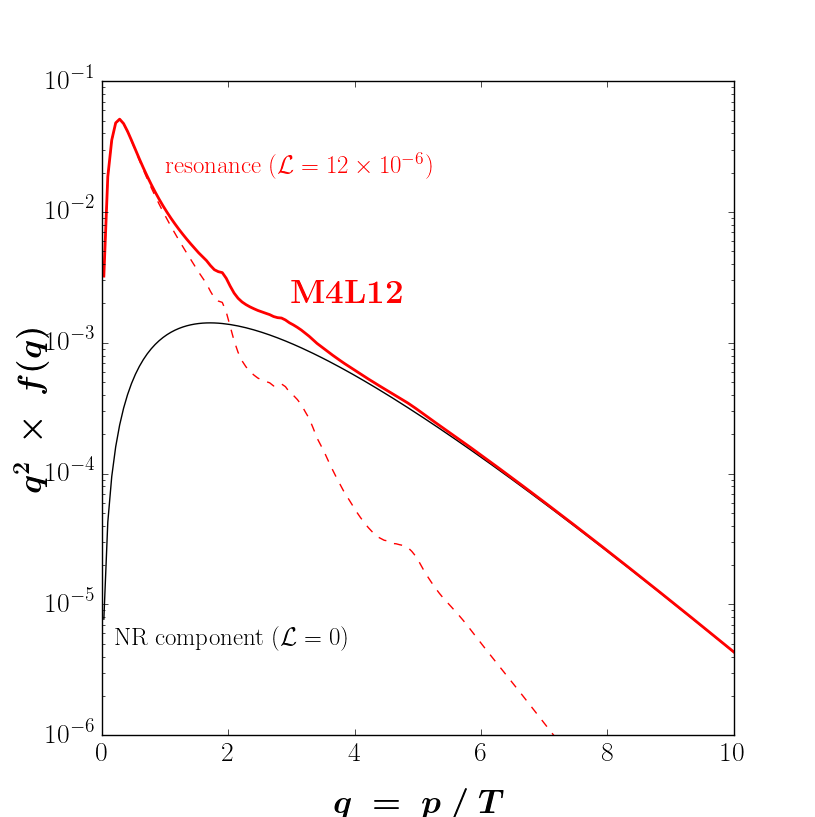
\includegraphics[width=0.55\columnwidth]{RPSN/RPSN_M4L12_psd.png}~%
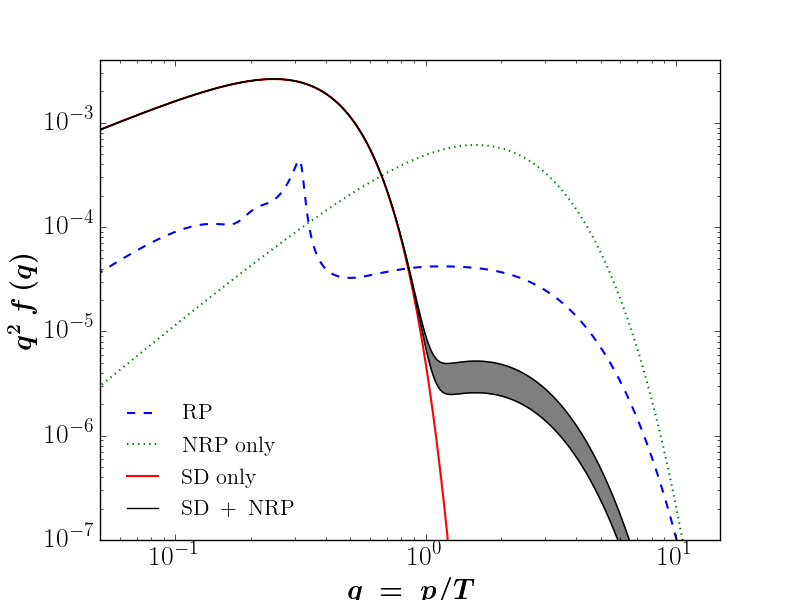
\includegraphics[width=0.55\columnwidth]{RPSN/SD.png}
\caption{\textbf{Left:} Distribution function of a $m_{\nu_s} = 4~\mathrm{keV}$ sterile neutrino produced via oscillations in presence of a net lepton asymmetry of $\mathcal{L} = 1.2 \times 10^{-5}$ (red solid curve labeled `M4L12'). The purely resonant component is featured in dashed red to distinguish it from the non-resonant component in solid black. \textbf{Right:} Distribution functions of $m_{\nu_s} = 7.1~\mathrm{keV}$ sterile neutrinos produced non-resonantly (dotted green curve labeled `NRP'), resonantly (dashed blue curve labeled `RP') and by the decay of a scalar field (red and black solid curves).}
\label{fig:M4L12_fs}
\end{center}
\end{figure}


As \cite{ShiFuller99} point out, the production of right-handed neutrinos via oscillations with the left-handed ones can be significantly boosted if one assumes a net lepton asymmetry in the Early Universe. The chemical potential term $\mu > 0$ in Eq.~\ref{eq:fs} can reach orders of $\mu \sim 10^{-4}$. The resulting distribution function of these \textbf{resonantly produced sterile neutrions} (RPSN) can end up being highly non-thermal, such as the one featured in red on the left panel of Fig.~\ref{fig:M4L12_fs} (also the dashed blue curve on the right panel ), produced in presence of a net lepton\footnote{I assume the lepton asymmetry to be mainly of the electronic charge, although there may be muonic and tauic charge asymmetries as well.} asymmetry of $\mathcal{L} = 1.2 \times 10^{-5}$ where $\mathcal{L}$ is the numerical density asymmetry of electronic neutrinos in units of entropy density:
\begin{equation}
\mathcal{L} = \frac{\left\vert n_{\nu_e} - n_{\bar{\nu}_e} \right\vert}{s}
\end{equation} To be consistent with light element abundances from big bang nucleosynthesis (BBN), this electronic asymmetry cannot exceed $\mathcal{L} \sim 10^{-3}$. However, asymmetries 3 orders of magnitude fainter than that upper limit can produce a significant resonance peak manifest in the distribution functions of RPSN. As such, RPSN are distributed with lower momenta than the quasi-thermally distributed NRP sterile neutrinos. If one assumes these neutrinos make up the dark matter, or part of it, then one can produce them with much weaker interaction angles $\theta$ for a fixed $\Omega_{\nu_s} \sim \Omega_{\mathrm{dm}}$ compared to Eq.~\ref{eq:fs}. \\

In this thesis, I consider left-handed and right-handed neutrinos as dark matter candidate particles. For the latter, I only consider ones produced via the oscillation mechanism, either in presence or absence of a net lepton asymmetry at the era of peak production. It should be noted, nevertheless, that ample other production mechanisms exist, which can all yield non thermal distributions typically cooler than the NRP case. Aside from the aforementioned NRP and RP production, neutrinos can be produced by the \textbf{decay of a scalar field}, initially proposed by \cite{Scalar_Decay3} and investigated by \cite{Scalar_Decay1, Scalar_Decay2, Scalar_Decay4}. The first numerical results were produced by \cite{Scalar_Decay_Merle}. The right panel of Fig.~\ref{fig:M4L12_fs} features the excess of momenta states populated in this production mechanism, where the position of the peak is linked to the scalar field particle's mass. Another noteworthy production mechanism is \textbf{thermal overproduction} with a subsequent entropy dilution, first put forth by \cite{thermal_overproduction} and reviewed in \cite{KingMerle}. The object of my thesis isn't to explore the plethera of production mechanisms, however, and I limit this current discussion to only the main axes of research on this topic. \\

Regardless of the production mechanism, the integral of the distribution function over all momenta yields the departure from the effective number of stable relativistic thermalized species in the early Universe from its fiducial value of $N_{\mathrm{eff}} = 3.046$: \\
\begin{equation}
\int \frac{dq}{2 \pi^2} q^2 f_s (q) = \frac{7}{8} \frac{\pi^2}{15}~T^4_\nu~\Delta N_{\mathrm{eff}}
\end{equation} \\To be consistent with the currently allowed bound on $N_{\mathrm{eff}}$ in Eq.~\ref{eq:neff_cmb}, the value of the normalisation parameter $\vartheta$ of the NRP sterile neutrinos' distribution function in Eq.~\ref{eq:fs} must not be of order unity. Typically, $\vartheta = \sin^2 2 \theta \simeq 10^{-7}$ for a NRP sterile neutrino of rest mass $m_{\nu_s} \sim \mathrm{keV}$ can account for $\Omega_{\mathrm{dm}} \simeq 0.26$ (see Sec.~\ref{sec:dmintro}). For a RPSN of the same mass, $\vartheta \simeq 10^{-12}$ can yield that same energy density and the same $\Delta N_{\mathrm{eff}}$. 








\subsection{Inventory of Non-Relativistic Matter}

I now instantiate the non-relativistic matter population, which in sum total have an energy density of \\
\begin{empheq}[box=\mymath]{equation}
\label{eq:omega_matter}
\Omega_{m} = 0.26142
\end{empheq} \\ critical densities today, and are subdivided into three categories: (1) everything made of atoms, including stars, dust and gas, (2) everything that has mass but isn't made of atoms, \emph{dark matter}, and (3) black holes. Leaving aside the third category, I detail the first two in the following two subsections. When matter is the dominant component in terms of energy density, then the first Friedmann equation boils down to:\\

\begin{equation}
\label{eq:Friedmann_MDE}
\left( \frac{\dot{a}}{a} \right)^2 \simeq \Omega_m = \Omega_{m,0} ~a^{-3}
\end{equation} \\ which integrates into $a(t) \propto t^{2/3}$ or equivalently $a(\tau) \propto \tau^{2}$ in terms of conformal time.


\subsubsection{Baryons and Acoustic Oscillations}
\label{sec:baos}

\begin{figure}
\centering
\begin{subfigure}{0.49\textwidth}
\centering
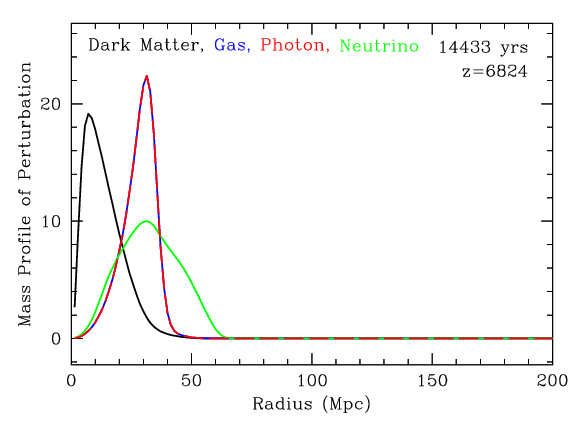
\includegraphics[width=\textwidth]{BAO/bao_z6824.png}
\caption{Near the initial time, the photons and baryons travel outward as a pulse.}\label{fig:bao_z6824}
\end{subfigure}
\hfill
\begin{subfigure}{0.49\textwidth}
\centering
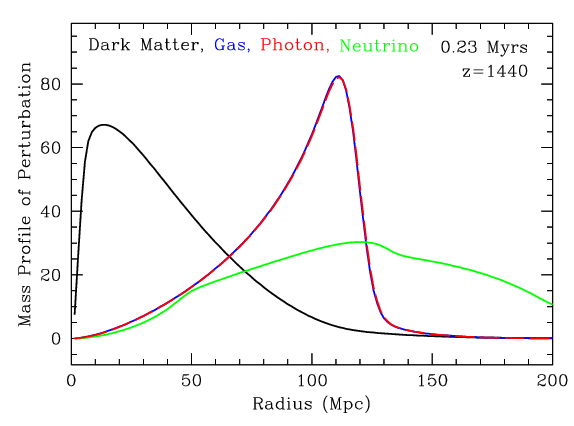
\includegraphics[width=\textwidth]{BAO/bao_z1440.png}
\caption{Approaching recombination, one can see the wake in the cold dark matter raised by the outward-going pulse of
baryons and relativistic species.}\label{fig:bao_z1440}
\end{subfigure}

\begin{subfigure}{0.49\textwidth}
\centering
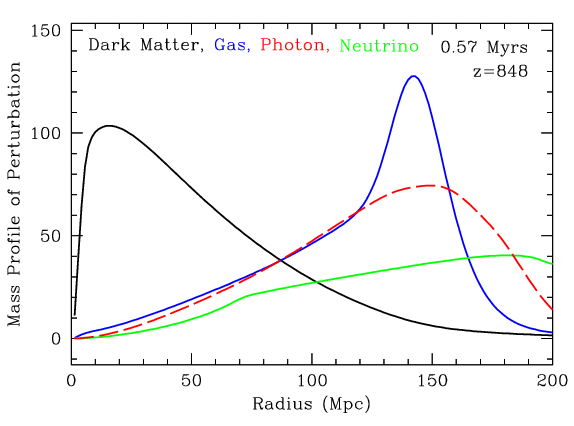
\includegraphics[width=\textwidth]{BAO/bao_z848.png}
\caption{At recombination, the photons leak away from the baryonic perturbation.}\label{fig:bao_z848}
\end{subfigure}
\hfill
\begin{subfigure}{0.49\textwidth}
\centering
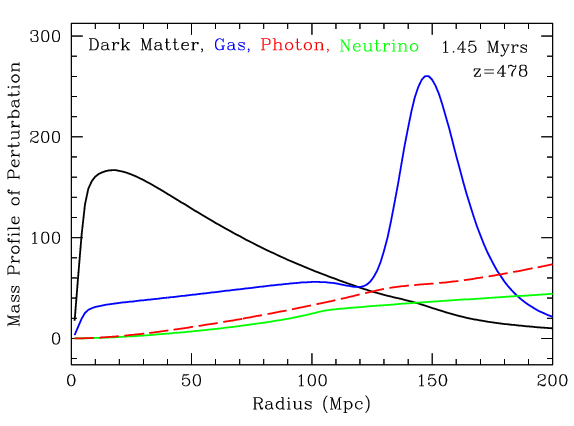
\includegraphics[width=\textwidth]{BAO/bao_z478.png}
\caption{With recombination complete, we are left with a dark matter perturbation toward the center and a baryonic
perturbation in a shell.}\label{fig:bao_z478}
\end{subfigure}

\begin{subfigure}{0.49\textwidth}
\centering
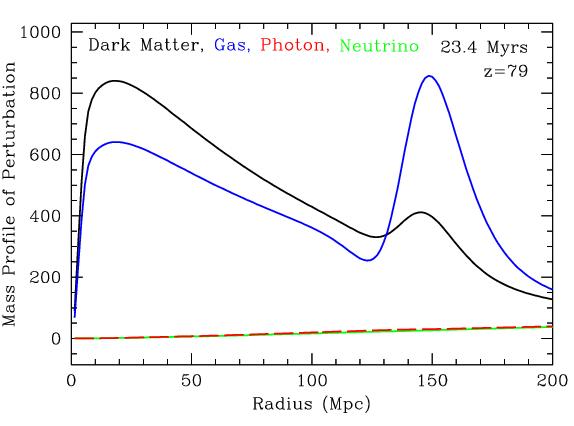
\includegraphics[width=\textwidth]{BAO/bao_z79.png}
\caption{Gravitational instability now takes over, and new baryons and dark matter are attracted to the overdensities.}
\label{fig:bao_z79}
\end{subfigure}
\hfill
\begin{subfigure}{0.49\textwidth}
\centering
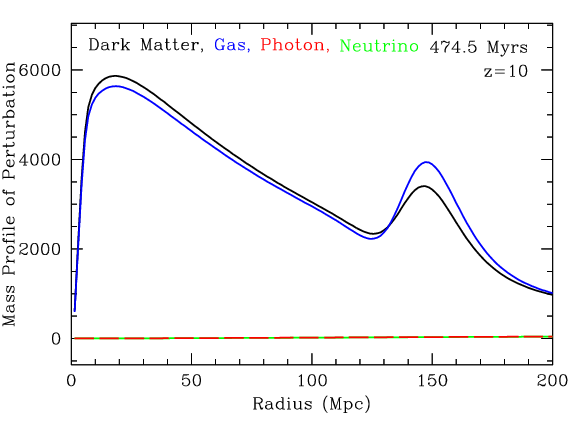
\includegraphics[width=\textwidth]{BAO/bao_z10.png}
\caption{The gas and dark matter peaks now look alike. The acoustic peak has decreased in contrast because dark matter,
which has no peak initially, outweighs the gas.}\label{fig:bao_z10}
\end{subfigure}

\caption{Evolution of the radial fractional mass profile versus comoving radius of an
initially pointlike overdensity located at the origin. The units of the mass profile are arbitrary but are correctly scaled between the 
panels. These figures were made by suitable transforms of the transfer functions created by \texttt{CMBFAST} \citep{Seljak1996, 
Zaldarriaga2000}. Credits: \citet{Eisenstein2007}.}\label{fig:bao_propagation}
\end{figure}

To distinguish ``regular'' matter from dark matter, any system made of atoms is refered to as \textbf{baryons}. Today, an obvious amount of baryons are bound to gravitational systems such as stars, planets, \textit{etc} due to growing density perturbations on very small scales. At larger scales, the interstellar and intergalactic media consist of hot tenous plasma containing a substancial amount of baryons from neutral atoms to ionized molecules. At earlier times, when the Universe was denser and hotter, the distribution of matter and baryons was much more uniform. When the Universe cools down to the binding energy of Hydrogen, electrons increasingly bind to protons to form neutral Hydrogen and photons scattering off the remaining free-electrons decreasingly. This \emph{recombination} occurs at around $z_{\mathrm{rec}} \simeq 1100$. Once about $90\%$ of the electrons are bound in neutral Hydrogen, photons last scatter off their ultimate free electron before free-streaming out and making the Universe transparent. At the redshift of this last scattering surface, $z_{\mathrm{lss}} \sim 1050$, the distribution of baryons is homogenous to within $\sim 10^{-5}$. The theory of structure formation relies mainly on gravitational instability, that is, the idea that in overdense regions, gravitational collapse overcomes the expansion. Thus overdensities tend to grow over time. In underdense regions on the other hand, the expansion is preponderant over their self-gravity and as such grow more underdense over time. \\

Before recombination, Thomson scattering between photons and electrons is predominant and the free-streaming scale of photons is much smaller than the size of the horizon $c H^{-1}(z)$. Photons and electrons are thus strongly coupled. This is known as the \emph{strong coupling limit}. In addition, protons and electrons interact through the Coulomb force. These three types of particles are coupled and form a unique
fluid called the baryon-photon plasma in which density perturbations evolve like sound waves. A point-like adiabatic perturbation in this baryon-photon plasma affects the dark matter, baryon, photon and neutrino populations. Neutrinos interact very weakly and stream away from the initial perturbation due to their high velocity. Dark matter is only affected by gravity and thus only stands growing at the original position. Because the baryon-photon plasma is
very hot and dominated by photons at this time, it has a strong pressure compared to its density. The initial overdensity is thus
also an initial overpressure. As the pressure tries to equalize itself with its surroundings, this results in an expanding spherical
sound wave, or \textbf{acoustic oscillation}, with the sound speed in the plasma $c_s \simeq c / \sqrt{3}$. The baryon and photon perturbation is carried outwards and its density drops as the energy is spread over the expanding
spherical wave as shown in Fig~\ref{fig:bao_z6824}. \\

As the acoustic wave propagates, the neutrinos free stream out and dark matter accumulates in the overall density
perturbation. Not only is the DM peak growing, but the width of the perturbation widens since it attracts additional material from its surroundings. This can be seen in Fig.~\ref{fig:bao_z1440}. Once recombination onsets, baryons decouple from the photons. The tight coupling limit is no longer valid and photons free stream like the neutrinos initially did at the onset of the perturbation, as shown on Fig.~\ref{fig:bao_z848}. Photons cool down and their pressure drops as the decoupling occurs, and thus the acoustic wave decelerates. This process continues until the photons have completely leaked out of the perturbation, and the sound wave has almost stopped
propagating. The remnants are a dark matter perturbation around the origin and a gas perturbation in a shell of about $\sim 150~\mathrm{Mpc}$ (comoving), seen in Fig.~\ref{fig:bao_z478}. However, baryons and dark matter interact gravitationally thus causing the two perturbations to feedback, \textit{i.e.} both increase due to the combined gravitational potential from both components (see Fig.~\ref{fig:bao_z79}). Eventually, the two perturbations look scarcely dissimilar and the spherical shell of gas has imprinted itself in the dark matter as the so-called acoustic peak (Fig.~\ref{fig:bao_z10}). \\

Since these perturbation are small in amplitude, the process just described can be linearly summed over the whole set of perturbation in the baryon-photon plasma. Galaxy formation occurs in overdense regions, and although most of it happens at the position of the original fluctuations, there is a tiny excess in the $\sim 150~\mathrm{Mpc}$ regions away from these initial perturbations. This length scale, originally related to a density
excess shortly after recombination, is expected to also be present in the distribution of matter in the later universe. It can
therefore be used as a standard ruler to probe our cosmological model. This is detected as a single \emph{acoustic peak} in the
correlation function of galaxies or a series of \emph{acoustic oscillations} in the corresponding power spectrum
\citep{Eisenstein2005,  Anderson2012}. Using this BAO scale and CMB anisotropies, we know baryons contribute \\
\begin{empheq}[box=\mymath]{equation}
\Omega_{b} h^2 = 0.022
\end{empheq} \\ to today's critical energy density.

\subsubsection{Dark Matter}
\label{sec:dmintro}

At the beginning of the 20th century, there appeared to be less light emaning from gravitationally-bound star clusters orbiting distant nebul{\ae}. Initially thought of as a ``missing light'' problem in which some material obstructed or occulted the light from these background sources, it became apparent a few decades later that it was in fact a ``missing mass'' issue. Indeed, if clouds of gas or dust in the foreground had absorbed the incoming light, then it should have manifested radiating as a black body at some wavelength. The mass from these luminous sources only accounted for one fifth of that required for these systems to be gravitationally bound and to reproduce their velocity dispersions. The other missing four fifths were hypothesized as an additional Dark Matter (DM), that has mass but neither absorbs nor emits nor scatters off light. In other words, dark matter is very little if at all sensitive to the electromagnetic interaction. \\

Although bold at the time, the postulation for the existence of dark matter has thus far stood the test of time. Other independant observations infer its presence: the non-Newtonian rotation curves of galaxies for one, but also the anisotropies in CMB temperatures, the BAOs described in the previous subsection, and gravitational lensing pictured in the right panel of Fig.~\ref{fig:bullet}. None of them outright prove its existence. However, dark matter neatly explains these independant observations. Ever since the advent of computational astrophysics in the 80's, numerical simulations have been unable to correctly reproduce the formation of structures and galaxies with ``ordinary'' matter only. All of the aforementioned cosmological probes for dark matter point to it having \\
\begin{empheq}[box=\mymath]{equation}
\Omega_{\mathrm{dm}} h^2 = 0.119
\end{empheq} \\ of today's critical energy density. Its nature however, is still unknown. If it is made of elementary particles, then images like the one in the left panel of Fig.~\ref{fig:bullet} suggest it can't be baryonic matter. When two galaxy clusters collide, the gas heats and radiates in the X-ray part of the spectrum, pictured as the pink overlay. The blue overlay points to where most of the mass distribution lies, as deduced by the gravitational lensing it exerts on the background light (an example of strong gravitational lensing is provided on the right panel). The pink and blue regions are clearly disparate, suggesting the area containing essentially all of the mass does not radiate. \\


\begin{figure}
\begin{center}
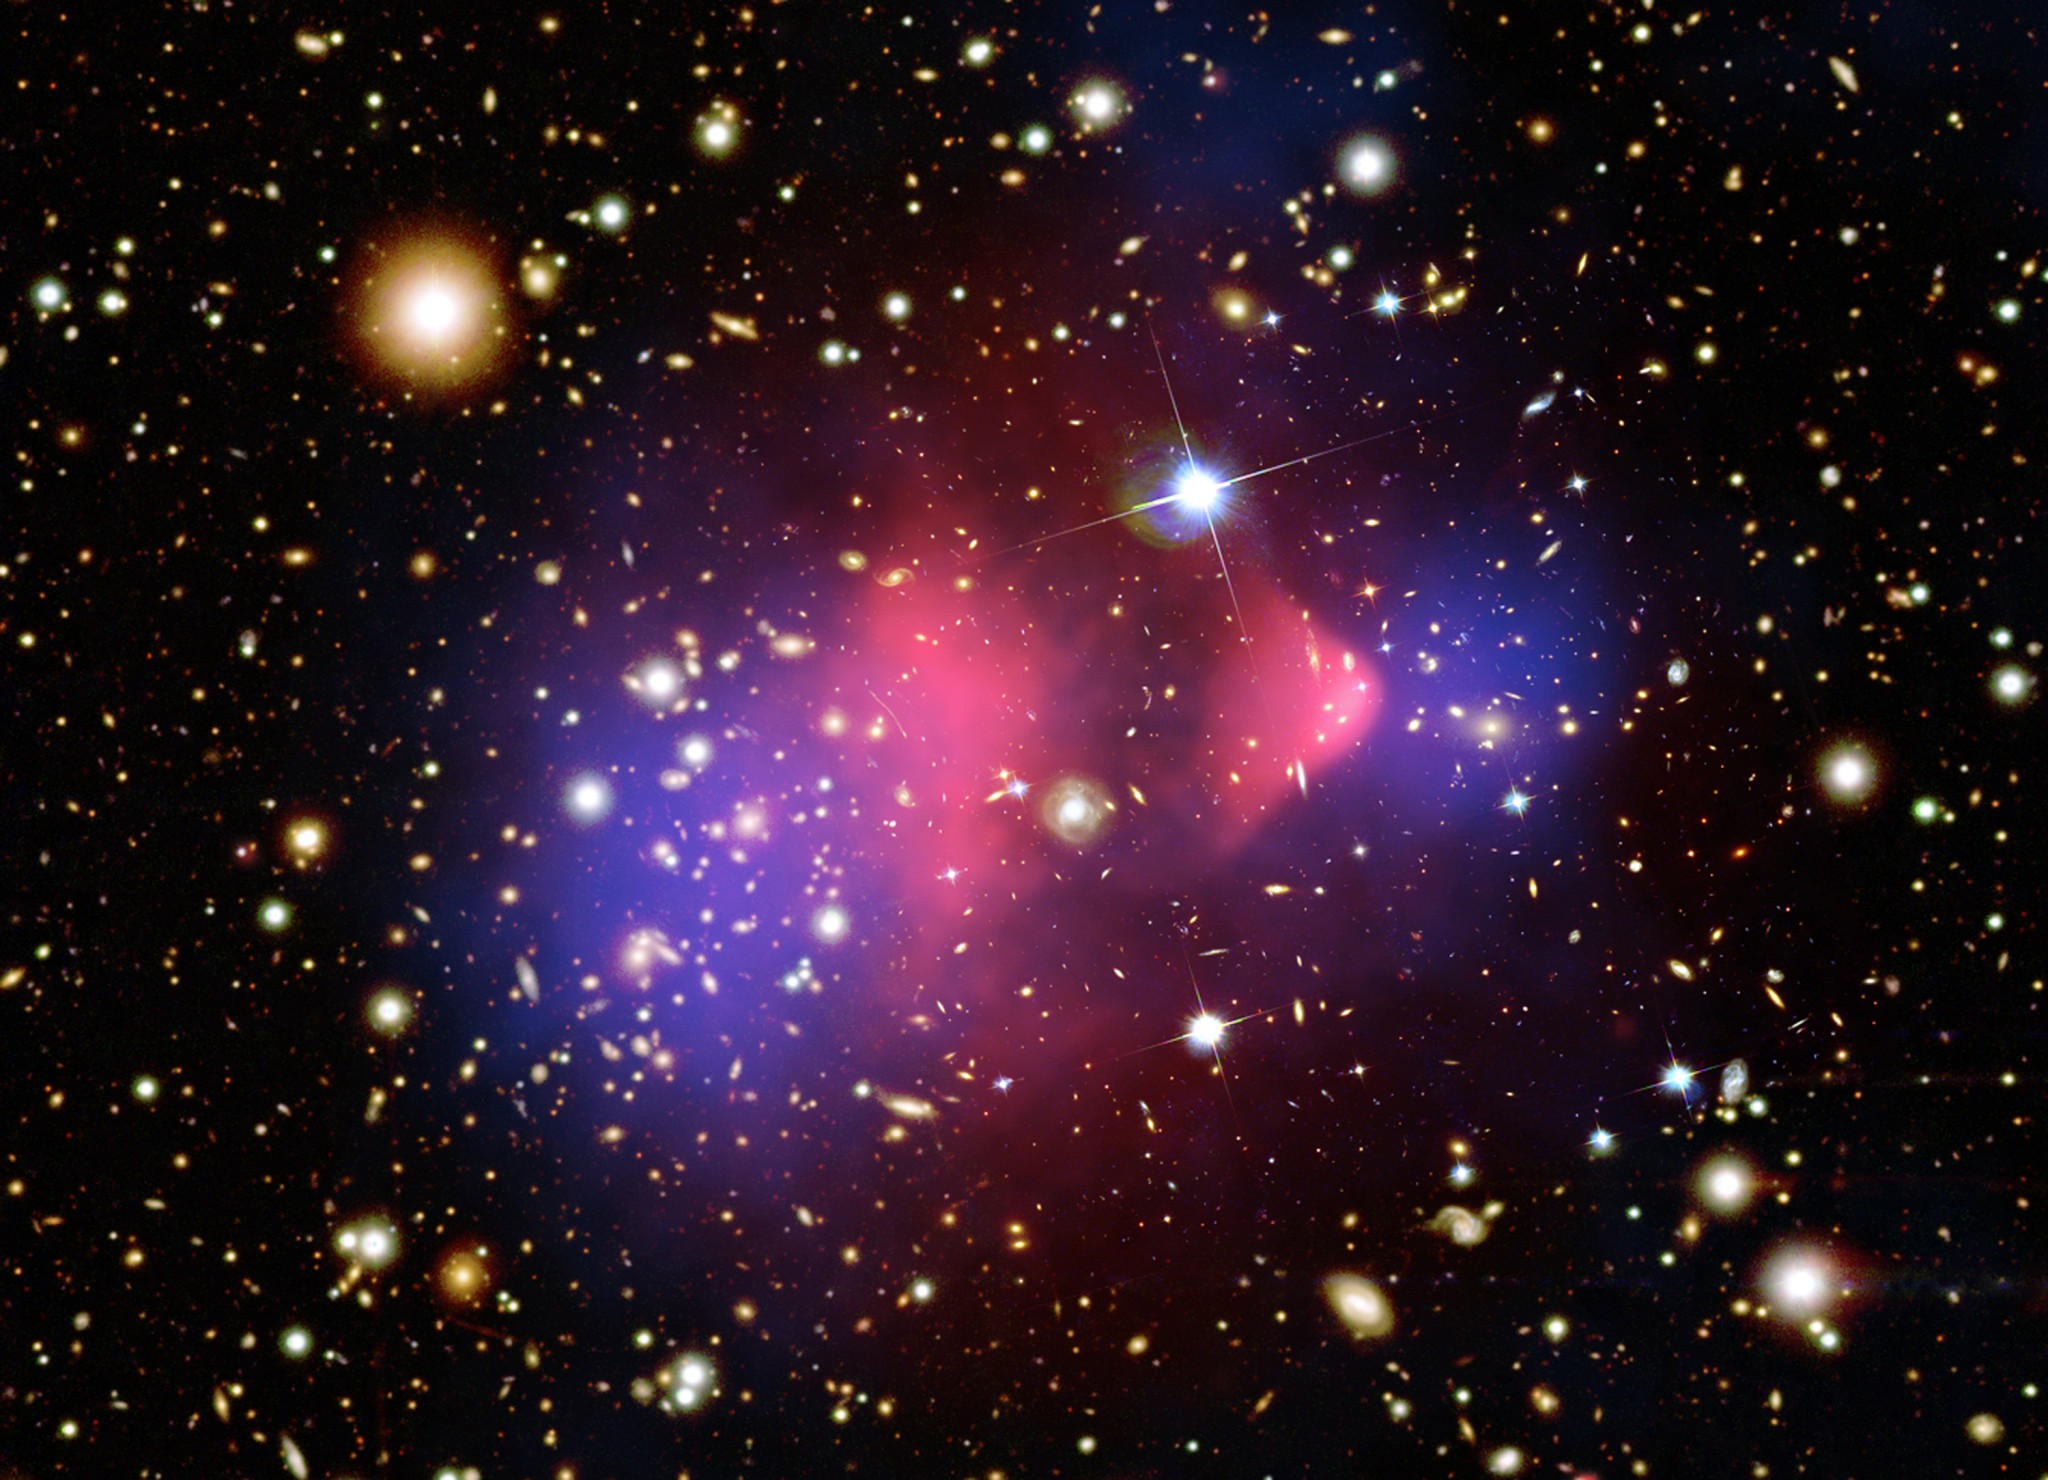
\includegraphics[height=5.5cm]{bulletcluster_comp_f2048.jpg}~%
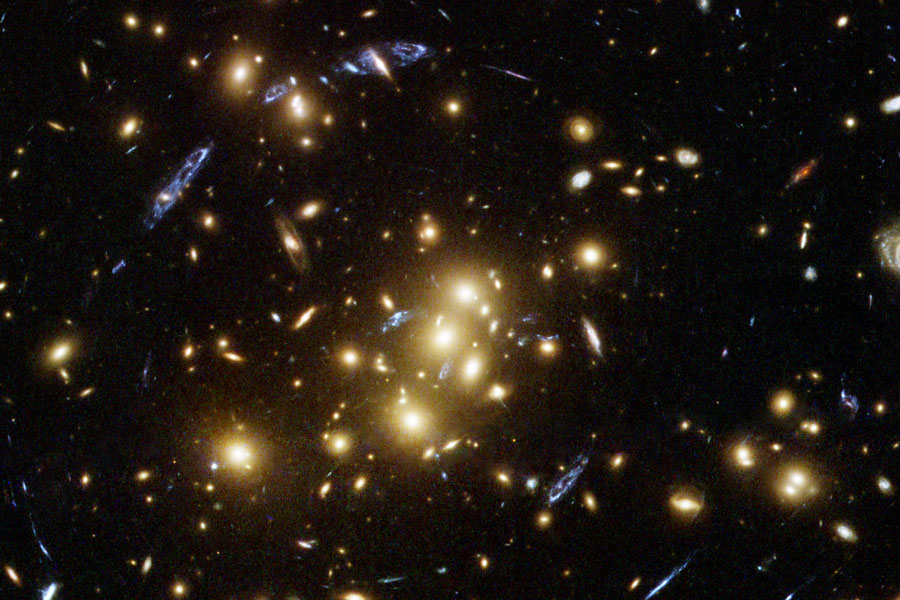
\includegraphics[height=5.5cm]{lentille-gravitationnelle.jpg}
\caption{\textbf{Left:} Composite optical image of the Bullet cluster, with X-ray in pink and weak gravitational lensing in blue (credit: NASA / STScI; ESO WFI; Magellan / U. of Arizona). \textbf{Right:} Gravitational lensing manifest near the 0024+1654 cluster (credit: HST), distorting the light rays from a background galaxy, shown as the stretched blue streaks.}
\label{fig:bullet}
\end{center}
\end{figure}

Despite the identity of a DM candidate particle still being speculative, it is nevertheless one of the most preponderant components of the Universe's energy density, second only to dark energy. As such, the current benchmark cosmological model is often refered to as the hot big bang $\Lambda$CDM model, where CDM stands for Cold Dark Matter. The ``cold'' adjective pertains to it having a narrow (quasi-Dirac) velocity distribution. In Sec.~\ref{sec:CAMB} in the next chapter, I distinguish cold dark matter from several non-cold dark matter cosmologies, the reason being that neutrinos --- the only DM candidate particle we've discovered --- cannot be cold as its velocity dispersion is to wide. This has a drastic impact on the formation of large scale structures and the distribution of the intergalactic gas, which I detail throughout this thesis.

\clearpage

\subsection*{Summary}

In an expanding Universe from a Hot Big Bang scenario described by a flat $\Lambda$CDM model, the expansion rate is driven by the energy density of a cosmological fluid through the Friedmann equations, which consists of three main components (radiation, matter and $\Lambda$) each having the following equations of state:\\

\begin{table}[!htbp]
	\begin{center}
		\begin{tabular}{cccc}
			\textbf{Component} & \textbf{Radiation} & \textbf{Matter} & \textbf{Dark Energy}\\[2pt]
			\hline \\[-10pt]
			Equation of State & $w_r = \cfrac{1}{3}$ & $w_m = 0$ & $w_\Lambda = -1$ \\[2pt]
			\hline \\[-10pt]
			Energy Density & $\rho_r \propto a^{-4}$ & $\rho_m \propto a^{-3}$ & $\rho_\Lambda \propto a^{0}$ \\[2pt]
			\hline \\[-10pt]
			Scale Factor & $a(t) \propto t^{1/2}$ & $a(t) \propto t^{2/3}$ & $a(t) \propto e^{H_0 \Omega_\Lambda^{1/2} t}$ \\[2pt]
			 & $a(\tau) \propto \tau$ & $a(\tau) \propto \tau^{2}$ & $a(\tau) \propto - 1/\tau$ \\[2pt]
			\hline \\[-10pt]
		\end{tabular}
	\end{center}
	%\label{tab:RDE_MDE}
\end{table}

In units of the critical energy density, the first Friedmann equation can be written: \\

\begin{equation}
\left( \frac{H(t)}{H_0} \right)^2 = \Omega^0_m a^{-3}(t) + \Omega^0_r a^{-4}(t) + \Omega^0_\Lambda
\end{equation} \\ This expression explicits the time dependance of the scale factor. Because the energy densities of these three components evolve distinctly with the scale factor, one can identify three epochs in the history of the Universe during which the radiation, matter and $\Lambda$ component dominates the others chronologically. One can determine when these epochs of domination swith from mainly radiation to mainly matter and finally to mainly $\Lambda$ (``matter - radiation equality'' and ``matter - $\Lambda$ equality'') by simply equating\\

\begin{align*}
\Omega_r (t) ~ a(t)^4 &= \Omega_r^0 ~ a_0^4\\
\Omega_m (t) ~ a(t)^3 &= \Omega_m^0 ~ a_0^3\\
\Omega_\Lambda (t) &= \Omega_\Lambda^0
\end{align*}\\

With today's values in Eqs.~\ref{eq:omega_lambda}, \ref{eq:omega_radiation} and \ref{eq:omega_matter}, one can straightforwardly compute that the cosmological constant dominates the dynamics of the observable Universe from $z=0$ to $z_\Lambda \simeq 0.3$. Prior to this redshift, the Universe was dominated by non-relativistic matter (matter dominated era or MDE) up to $z_{\mathrm{eq}} \simeq 3400$, prior to which was the radiation dominated era or RDE. Fig.~\ref{fig:cosmichistory} shows the evolution of $\Omega_r$, $\Omega_m$ and $\Omega_\Lambda$ with proper time, as well as that of the scale factor, and materializes the two equalities distinguishing the RDE from the MDE and the $\Lambda$DE. 

\begin{figure}
\begin{center}
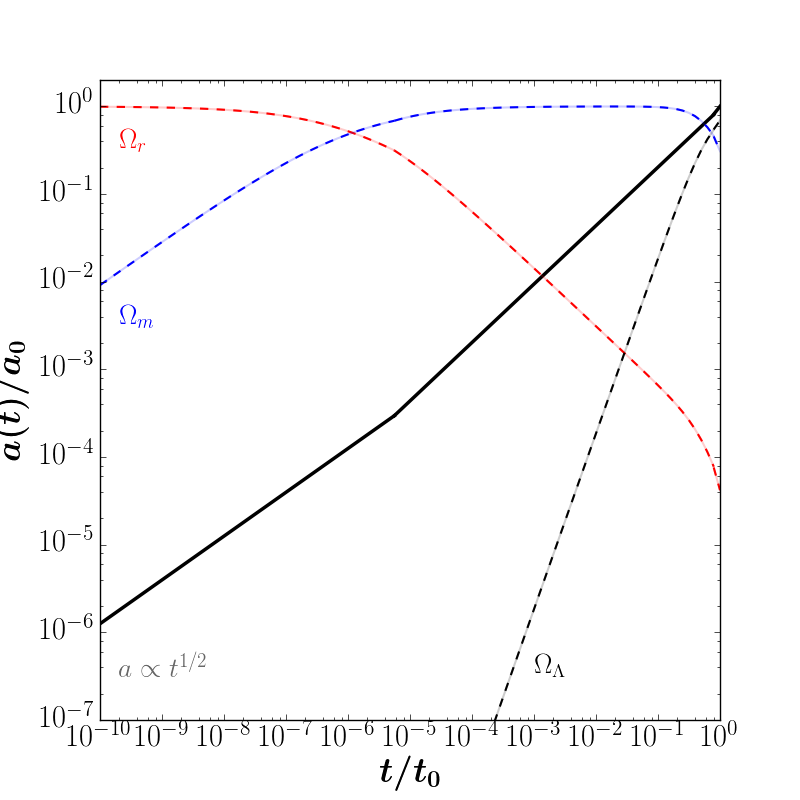
\includegraphics[width=0.75\columnwidth]{Cosmology/aa0.png}
\caption{Evolution of the radiation, matter and $\Lambda$ densities in units of critical density with respect to proper time (dot dashed color curves). The evolution of the scale factor in units of today's $a_0$ with proper time is superimposed as the solid black curve.}
\label{fig:cosmichistory}
\end{center}
\end{figure}

\clearpage